\section{Kết quả và bàn luận}\label{sec:04-evaluation-results}
\subsection{Chất lượng phân loại ảnh FP32}
Trên \ImageTest{} ảnh test, MobileNetV3-Large hiện tại đạt Accuracy \ImageAccuracy\% và macro-F1 \ImageMacroFOne\%. Balanced accuracy là 74,07\%. Ma trận nhầm lẫn và chất lượng từng lớp được trình bày ở Bảng~\ref{tab:confusion} và \ref{tab:image-classes}.
% Generated by scripts/export_results.py; do not edit.
\begin{table}[htbp]\centering\small

\caption{Ma trận nhầm lẫn model seed 1024: hàng thật, cột dự đoán}\label{tab:confusion}
\begin{tabular}{lrrrr}
\toprule
Nhãn & low & medium & high & non\_flood \\ \midrule
low & 34 & 14 & 0 & 8 \\
medium & 11 & 42 & 6 & 1 \\
high & 2 & 12 & 40 & 0 \\
non\_flood & 8 & 0 & 0 & 78 \\
\bottomrule\end{tabular}
\end{table}

% Generated by scripts/export_results.py; do not edit.
\begin{table}[htbp]\centering\small

\caption{Chất lượng model seed 1024 theo từng lớp}\label{tab:image-classes}
\begin{tabular}{lrrrr}
\toprule
Lớp & Precision (\%) & Recall (\%) & F1 (\%) & Số ảnh \\ \midrule
low & 61.82 & 60.71 & 61.26 & 56 \\
medium & 61.76 & 70.00 & 65.62 & 60 \\
high & 86.96 & 74.07 & 80.00 & 54 \\
non\_flood & 89.66 & 90.70 & 90.17 & 86 \\
\bottomrule\end{tabular}
\end{table}


Lớp \texttt{non\_flood} có recall 91,86\%, cao hơn các lớp ngập. Recall \texttt{high} là 66,67\%; trong 54 ảnh high, 14 ảnh bị dự đoán medium và 3 ảnh bị dự đoán low. Ranh giới giữa các mức ngập là hạn chế đáng chú ý, vì nhầm xuống mức thấp có thể làm metadata giảm mức ngập nếu không có kiểm chứng bổ sung.

Có 5 lỗi cách ít nhất hai mức severity, chiếm 1,95\% tập test. Đây là chỉ số do nhóm định nghĩa theo thứ tự mức ngập, không trực tiếp đo hệ quả cứu hộ. Số lượng test mỗi lớp còn nhỏ, nên chênh lệch vài ảnh làm tỷ lệ thay đổi đáng kể. Báo cáo chưa có khoảng tin cậy ghép cặp theo dữ liệu độc lập ngoài nguồn ảnh hiện tại để kết luận khác biệt nhỏ giữa các mô hình.

ECE của FP32 khoảng 0,06350 và Brier khoảng 0,34483 theo artifact. Các chỉ số này cung cấp thêm thông tin về confidence. Không dùng Accuracy tổng thể để chứng minh mọi dự đoán có confidence trên 0,90 đủ tin cậy cho quyết định không gửi ảnh; cần kiểm tra riêng nhóm quyết định đó và các ảnh ngoài phân bố.

\subsection{Tương đương PyTorch, ONNX và ExecuTorch}
% Generated by scripts/export_results.py; do not edit.
\begin{table}[htbp]\centering\small

\caption{So sánh ba định dạng mô hình trên cùng tập test}\label{tab:pth_onnx_pte}
\begin{tabular}{lrrrrr}
\toprule
Mô hình & Acc. (\%) & F1 (\%) & Lỗi nặng & MiB & Trung vị ms \\ \midrule
PyTorch FP32 & 76.17 & 74.54 & 5 & 48.51 & 65.87 \\
ONNX FP32 & 76.17 & 74.54 & 5 & 16.04 & 25.93 \\
ExecuTorch FP32 & 76.17 & 74.54 & 5 & 16.06 & 45.31 \\
\bottomrule\end{tabular}
\SourceNote{\RepoPath{products/fe/reports/pth_onnx_pte/summary.json}; 256 ảnh test, CPU máy tính; thời gian chỉ tính lời gọi suy luận.}
\end{table}

Cả ba định dạng có cùng nhãn top-1 trên 256 ảnh và cùng chỉ số phân loại. Sai khác xác suất tối đa PTH--ONNX khoảng $3{,}01\times10^{-6}$; PTH--PTE khoảng $5{,}01\times10^{-6}$. Kết quả cho thấy chuyển đổi FP32 giữ đầu ra tốt trên split được đo với pipeline đã khai báo.

Trong phiên này, trung vị lời gọi suy luận PTH là 65,87 ms, ONNX 25,93 ms và PTE 45,31 ms. File checkpoint PTH khoảng 48,51 MiB, ONNX 16,04 MiB và PTE 16,06 MiB. Đây là đối chiếu trên máy tính, không đủ để chọn runtime nhanh nhất trên mọi điện thoại. Kích thước PTH lớn hơn không có nghĩa toàn bộ phần chênh lệch là tham số tính toán cần cắt tỉa.

Smoke verification trên ba ảnh ghi năm kiểm tra local pass gồm tiền xử lý, precision, provider, parity và label mapping; phần mobile ghi chưa thử. Kết quả smoke hỗ trợ kiểm tra đường thực thi nhỏ, còn kết quả full test hỗ trợ thống kê phân loại. Hai mức kiểm tra bổ sung nhau và không thay thế phép đo pixel/runtime native trên điện thoại.

\subsection{Lượng tử hóa: số liệu đã lưu và đối chiếu chưa khớp}
Bảng lượng tử hóa dưới đây giữ số từ \texttt{summary.json} để truy nguyên artifact, chưa xem là metric nén được xác nhận cuối cùng. Khi tính lại từ \texttt{all\_predictions.csv} cùng thư mục, PTQ có một khác biệt ở ma trận nhầm lẫn và QAT có ba dự đoán đúng ít hơn summary. Bảng~\ref{tab:image-metric-audit} công bố cả hai nguồn; nguyên nhân cần được rà soát ở quy trình sinh artifact.
% Generated by scripts/export_results.py; do not edit.
\begin{table}[htbp]\centering\small
\setlength{\tabcolsep}{3pt}
\caption{Đối chiếu các số liệu summary chưa khớp CSV dự đoán}\label{tab:image-metric-audit}
\begin{tabular}{lrrrr}
\toprule
Mô hình & \shortstack{Acc. summary\\(\%)} & \shortstack{Acc. CSV\\(\%)} & \shortstack{F1 summary\\(\%)} & \shortstack{F1 CSV\\(\%)} \\ \midrule
ptq\_int8 & 71.88 & 71.88 & 70.33 & 70.34 \\
qat\_int8 & 52.34 & 51.17 & 50.57 & 49.19 \\
\bottomrule\end{tabular}
\SourceNote{\RepoPath{products/fe/reports/fp32_ptq_qat/summary.json} và all\_predictions.csv cùng thư mục; giữ nguyên hai nguồn, chưa chốt metric nén.}
\end{table}

% Generated by scripts/export_results.py; do not edit.
\begin{table}[htbp]\centering\small

\caption{PTQ/QAT theo summary đã lưu; số liệu nén cần rà soát}\label{tab:fp32_ptq_qat}
\begin{tabular}{lrrrrr}
\toprule
Mô hình & Acc. (\%) & F1 (\%) & Lỗi nặng & MiB & Trung vị ms \\ \midrule
ONNX FP32 & 76.17 & 74.54 & 5 & 16.04 & 31.90 \\
PTQ INT8 & 71.88 & 70.33 & 5 & 4.51 & 35.37 \\
QAT INT8 & 52.34 & 50.57 & 38 & 4.57 & 121.36 \\
\bottomrule\end{tabular}
\SourceNote{\RepoPath{products/fe/reports/fp32_ptq_qat/summary.json}; 256 ảnh test, CPU máy tính; thời gian chỉ tính lời gọi suy luận.}
\end{table}

PTQ INT8 giảm file ONNX từ khoảng 16,04 xuống 4,51 MiB, xấp xỉ 71,9\% dung lượng theo byte của artifact. Accuracy giảm từ 76,17\% xuống 71,88\%, tương ứng khoảng 4,30 điểm phần trăm. Macro-F1 giảm từ 74,54\% xuống 70,33\%. Top-1 agreement với FP32 bằng 86,72\%, nên việc nén thay đổi một phần dự đoán.

Trong phiên đo FP32/PTQ/QAT, trung vị PTQ 35,37 ms cao hơn FP32 31,90 ms. Artifact lượng tử hóa riêng có trung vị khác vì phiên đo khác; báo cáo không chọn số thuận lợi ở phiên khác để khẳng định INT8 luôn nhanh hơn. Kết luận có căn cứ ở đây là giảm dung lượng kèm đánh đổi chất lượng, còn lợi ích tốc độ phụ thuộc runtime/hardware.

Theo summary đã lưu, QAT INT8 của nhánh hiện tại đạt Accuracy 52,34\%, macro-F1 50,57\% và 38 lỗi nặng (14,84\%). Trung vị 121,36 ms cao hơn hai đối chứng trong cùng phiên. Đây là kết quả không thuận lợi của nhánh QAT đã lưu, cần giữ trong báo cáo. Không suy ra QAT nói chung luôn kém; phép đo chỉ đặc trưng cho checkpoint và quy trình hiện tại, và chưa cô lập được nguyên nhân suy giảm.

\subsection{Cắt tỉa có cấu trúc}
% Generated by scripts/export_results.py; do not edit.
\begin{table}[htbp]\centering\small

\caption{Đối chiếu trước và sau cắt tỉa có cấu trúc}\label{tab:pruning_st}
\begin{tabular}{lrrrrr}
\toprule
Mô hình & Acc. (\%) & F1 (\%) & Lỗi nặng & MiB & Trung vị ms \\ \midrule
PTH gốc & 76.17 & 74.54 & 5 & 48.51 & 33.16 \\
PTH cắt tỉa & 76.17 & 74.47 & 4 & 16.06 & 28.91 \\
ONNX gốc & 76.17 & 74.54 & 5 & 16.04 & 12.71 \\
ONNX cắt tỉa & 76.17 & 74.47 & 4 & 15.81 & 20.32 \\
PTE gốc & 76.17 & 74.54 & 5 & 16.06 & 25.62 \\
PTE cắt tỉa & 76.17 & 74.47 & 4 & 15.83 & 32.43 \\
\bottomrule\end{tabular}
\end{table}

Artifact ghi số tham số giảm từ 4.207.156 xuống 4.145.694, khoảng 1,46\%. File ONNX giảm từ 16,04 xuống 15,81 MiB; PTE giảm từ 16,06 xuống 15,83 MiB. Accuracy giữ ở 76,17\%, macro-F1 thay đổi nhẹ từ 74,54\% xuống 74,47\%, và số lỗi nặng giảm từ 5 xuống 4.

Cùng Accuracy không có nghĩa cùng dự đoán: đồng thuận giữa mô hình gốc và cắt tỉa chỉ 81,64\% trên tập test. Một số ảnh chuyển từ đúng sang sai, trong khi ảnh khác chuyển từ sai sang đúng. Vì vậy cần nhìn per-class và disagreement thay vì chỉ một tỷ lệ tổng.

Về tốc độ trong cùng phiên, PTH cắt tỉa có trung vị thấp hơn PTH gốc (28,91 so với 33,16 ms), nhưng ONNX cắt tỉa cao hơn (20,32 so với 12,71 ms) và PTE cắt tỉa cao hơn (32,43 so với 25,62 ms). Ít tham số hơn không bảo đảm runtime nhanh hơn, vì kernel, bố trí graph và backend có thể khác. Chưa có nhiều lần đo độc lập hoặc kết quả mobile để khẳng định ưu thế hiệu năng tổng quát.

\subsection{Khẩn cấp LR: độ khớp nhãn thay thế}
JSON v5 ghi fidelity trên 32 trạng thái tại threshold 0,5 bằng 1,0. Bảng so sánh với quy tắc cho thấy tất cả profile khớp nhãn OR. Các audit dataset/final gate ghi kiểm tra integrity; audit nguồn giữ các trạng thái có điều kiện và thay đổi sau rà soát, không chuyển mọi hạng mục thành một phát biểu ``pass'' vô điều kiện.

Sanity 10 vòng giữ một số profile dương để kiểm tra khả năng dự đoán trạng thái chưa có trong train của vòng đó. Có vòng recall 0,75 hoặc 0,667, nên không nên diễn giải kết quả toàn bảng là tổng quát hoàn hảo khi huấn luyện thiếu profile. Đây là kiểm tra kỹ thuật trong không gian tổng hợp hữu hạn. Mô hình không được đánh giá trên người bệnh, tin nhắn tự do hoặc dữ liệu điều phối thực.

Phần app đã có loader và score từ cờ có cấu trúc, nhưng backend vẫn dùng trường \texttt{urgency}/từ khóa khi phân cụm. Vì vậy, mức hoàn thành của gói LR là có dữ liệu, mô hình, audit và đường tính tại app; chuỗi app--adapter--đồ thị dùng $E_i^{\mathrm{LR}}$ cần thêm kiểm thử tích hợp. Đây cũng là lý do không gọi hệ thống hiện tại đã hoàn tất mô hình văn bản đa phương thức.

\subsection{RQ1: chất lượng phân cụm cơ sở}
% Generated by scripts/export_results.py; do not edit.
\begin{table}[htbp]\centering\small

\caption{Kết quả RQ1 trên 40 run test của Generator 3.0}\label{tab:rq1-benchmark}
\begin{tabular}{lrrr}
\toprule
Phương pháp & ARI [CI 95\%] & Pair F1 & ĐK cụm (km) \\ \midrule
Additive Louvain & 0.9191 [0.8995; 0.9381] & 0.9247 & 0.3477 \\
Product Leiden & 0.9165 [0.8979; 0.9351] & 0.9223 & 0.3547 \\
Convex Louvain & 0.9135 [0.8940; 0.9320] & 0.9195 & 0.3547 \\
Product Louvain & 0.9072 [0.8864; 0.9271] & 0.9138 & 0.3585 \\
Additive mật độ khớp & 0.8973 [0.8763; 0.9175] & 0.9046 & 0.3743 \\
K-means tọa độ & 0.8176 [0.7976; 0.8384] & 0.8292 & 0.2977 \\
Gom cụm phân cấp & 0.6235 [0.5964; 0.6494] & 0.6506 & 4.1648 \\
HDBSCAN & 0.5205 [0.4565; 0.5811] & 0.5787 & 1.2527 \\
Geo-time DBSCAN & 0.4978 [0.4589; 0.5366] & 0.5450 & 0.6244 \\
DBSCAN mọi đặc trưng & 0.4741 [0.4273; 0.5201] & 0.5488 & 0.9340 \\
\bottomrule\end{tabular}
\SourceNote{\RepoPath{thucnghiem/results/cij_baseline_benchmark_results/benchmark_summary.csv}; đường kính trung bình chỉ là thống kê mô tả.}
\end{table}

Additive Louvain có ARI trung bình 0,9191, cao nhất bảng; Product Louvain là 0,9072. Product trừ Additive được chọn độc lập có hiệu trung bình $-0{,}01184$, CI bootstrap 95\% chưa hiệu chỉnh $[-0{,}02257;-0{,}00240]$, với 9 run thắng, 19 hòa và 12 thua. Wilcoxon raw $p=0{,}0987$, sau Holm $p=0{,}2560$. Kết quả không xác lập ưu thế thành phần tích.

So với Additive khớp mật độ, Product có hiệu $+0{,}00989$, CI $[-0{,}00100;0{,}02082]$ và $p_{\mathrm{Holm}}=0{,}2560$. Hai pipeline có retained-edge fraction xấp xỉ 0,03011 và 0,03021, mean degree 9,90 và 9,94. Đây là diagnostic giảm chênh lệch mật độ, không xác định tác động nhân quả của operator, vì trọng số và thành viên cạnh vẫn khác.

Product Leiden có ARI 0,9165; phép so sánh với Product Louvain sau Holm có $p=0{,}1120$. Các kết quả cho thấy cần đánh giá cả cấu hình đồ thị và bộ phát hiện cộng đồng. Các baseline mật độ thấp hơn trong bundle này không chứng minh chúng kém trong mọi môi trường hoặc mọi cách chuẩn hóa đặc trưng.

Một phát hiện vận hành là Product có fake absorption và fake rejection đều bằng không, nhưng false-destination rate 16,49\%. Tin giả không hòa vào điểm thật nhưng tạo điểm đến giả riêng. Vì thế, tỷ lệ hấp thụ bằng không không được gọi là chống tin giả hiệu quả. Nếu scheduler coi các cụm giả là điểm cần đi, chúng vẫn tiêu tốn nguồn lực.

\subsection{RQ1: độ nhạy dưới nhiễu và bản sao}
% Generated by scripts/export_results.py; do not edit.
\begin{table}[htbp]\centering\small

\caption{ARI dưới nhiễu cố định; đánh giá trên báo cáo gốc có liên kết sự kiện}\label{tab:rq1-stress}
\begin{tabular}{lrrrr}
\toprule
Điều kiện & Product & Additive & Leiden & DBSCAN \\ \midrule
Đối chứng & 0.9072 & 0.9191 & 0.9165 & 0.4978 \\
GPS 100 m & 0.8956 & 0.8971 & 0.9047 & 0.4678 \\
GPS 300 m & 0.7816 & 0.7626 & 0.7912 & 0.3709 \\
Thời gian 15 phút & 0.8722 & 0.8815 & 0.8850 & 0.4856 \\
Thời gian 60 phút & 0.7442 & 0.7646 & 0.7604 & 0.4432 \\
Bản sao $2\times$ & 0.9314 & 0.9337 & 0.9313 & 0.4978 \\
Bản sao $5\times$ & 0.2964 & 0.2971 & 0.2964 & 0.4978 \\
\bottomrule\end{tabular}
\end{table}

\begin{figure}[htbp]\centering
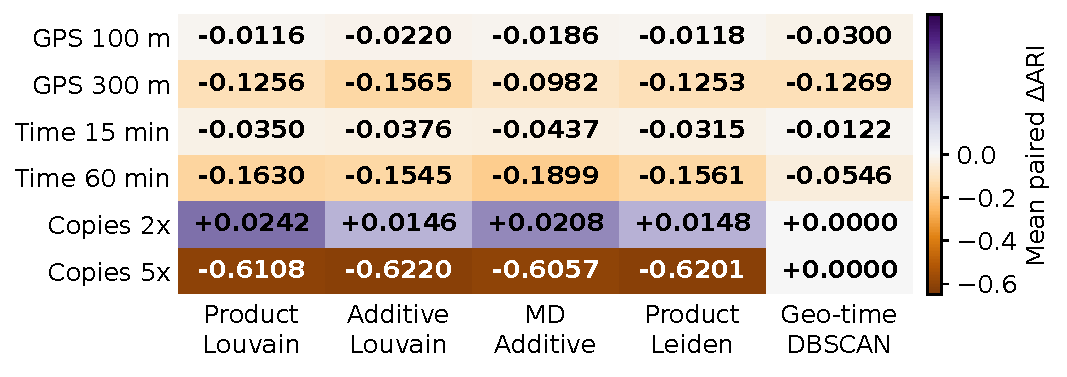
\includegraphics[width=.97\textwidth]{../paper/figures/rq1_stress_delta_ari.pdf}
\caption{Thay đổi ARI trong từng phương pháp so với đối chứng, 40 run test RQ1}
\label{fig:rq1-stress-report}
\end{figure}
\SourceNote{\RepoPath{paper/figures/rq1_stress_delta_ari.pdf}; nguồn chính \RepoPath{thucnghiem/results/rq1_results/aggregate/}. Giá trị âm biểu diễn suy giảm; không phải kiểm định ưu thế giữa phương pháp.}

Các mức nhiễu tọa độ và thời gian được thử đều làm ARI trung bình giảm. Không phương pháp nào đứng đầu ở mọi điều kiện. Bản sao hai lần làm ARI của bốn biến thể đồ thị tăng nhẹ, nhưng năm lần làm trung bình về khoảng 0,30. Geo-time DBSCAN giữ mức đối chứng thấp hơn khi chỉ thay multiplicity exact.

Với Product Louvain, thay đổi năm lần là $-0{,}6108$, CI ghép cặp chưa hiệu chỉnh $[-0{,}6318;-0{,}5881]$. Hai multiplicity được thử cho thấy đáp ứng không đơn điệu, không xác định một ngưỡng sụp đổ chính xác và không chứng minh thêm bản sao có lợi. Quantile và cạnh top-$k$ là các cơ chế có thể liên quan, nhưng protocol chưa cô lập nguyên nhân.

Lần chạy độc lập không gộp chỉ làm một số tổng hợp ở điều kiện hai lần khác nhẹ; kết luận GPS, timestamp và năm lần được giữ theo audit. Quan trọng hơn, thất bại ở phân cụm cùng tồn tại với bất biến sao chép của score khi grouping cố định. Hai phát biểu áp dụng hai tầng khác nhau.

\subsection{RQ2: phù hợp với lợi ích mô phỏng}
% Generated by scripts/export_results.py; do not edit.
\begin{table}[htbp]\centering\small

\caption{NDCG@5 với nhóm sự kiện oracle trên 40 seed Candidate 4.1}\label{tab:rq2-alignment}
\begin{tabular}{lrr}
\toprule
Điểm xếp hạng & NDCG@5 & CI 95\% \\ \midrule
Điểm có chặn & 0.6669 & [0.6306; 0.7018] \\
Legacy & 0.6548 & [0.6229; 0.6850] \\
Chỉ số người & 0.6709 & [0.6471; 0.6955] \\
Ngẫu nhiên & 0.6763 & [0.6405; 0.7100] \\
Tuyến tính & 0.6448 & [0.6127; 0.6759] \\
Chỉ khẩn cấp & 0.6352 & [0.6057; 0.6641] \\
\bottomrule\end{tabular}
\SourceNote{\RepoPath{thucnghiem/results/rq2_results/rq2_summary.csv}; nhóm oracle chỉ dùng cho chẩn đoán riêng tầng xếp hạng.}
\end{table}

Điểm có chặn đạt NDCG@5 0,6669, CI 95\% $[0{,}6306;0{,}7018]$. Spearman trung bình $-0{,}0304$ với CI $[-0{,}1165;0{,}0549]$, overlap top-5 bằng 0,285 với CI $[0{,}2349;0{,}3400]$. NDCG@5 cao hơn legacy khoảng 0,0121 nhưng tương phản sau Holm không có ý nghĩa theo artifact.

Ước lượng điểm của phương pháp có chặn còn thấp hơn chỉ số người (0,6709) và ngẫu nhiên (0,6763). Những chênh lệch điểm này không tự chứng minh khác biệt thống kê. Vì grouping oracle đã loại lỗi phân cụm khỏi điều kiện RQ2, sự phù hợp yếu không thể quy hoàn toàn cho phân hoạch sai.

\subsection{RQ2: bất biến hẹp và thất bại dưới phối hợp}
% Generated by scripts/export_results.py; do not edit.
\begin{table}[htbp]\centering\small
\setlength{\tabcolsep}{3pt}
\caption{Độ nhạy RQ2: R là score có chặn, L là legacy; thấp hơn là tốt hơn}\label{tab:rq2-robustness}
\begin{tabular}{lrrrrrr}
\toprule
Điều kiện & $\Delta P_R$ & $\Delta P_L$ & $\Delta r_R$ & $\Delta r_L$ & Churn R & Churn L \\ \midrule
Mâu thuẫn $F/E$ & 0.0484 & 0.0611 & 0.0171 & 0.0290 & 0.0450 & 0.1100 \\
Phối hợp confidence cao & 0.1688 & 0.0309 & 0.0175 & 0.0006 & 0.0350 & 0.0000 \\
Exact $10\times$ & 0.0000 & 0.0148 & 0.0000 & 0.0075 & 0.0000 & 0.0150 \\
Exact $2\times$ & 0.0000 & 0.0026 & 0.0000 & 0.0015 & 0.0000 & 0.0000 \\
Exact $5\times$ & 0.0000 & 0.0086 & 0.0000 & 0.0046 & 0.0000 & 0.0100 \\
Tăng $E$, confidence thấp & 0.0034 & 0.0012 & 0.0008 & 0.0006 & 0.0050 & 0.0000 \\
Tăng $F$, confidence thấp & 0.0026 & 0.0072 & 0.0000 & 0.0040 & 0.0000 & 0.0150 \\
Tăng $N$, confidence thấp & 0.0696 & 0.0140 & 0.0240 & 0.0071 & 0.0600 & 0.0150 \\
Tăng $V$, confidence thấp & 0.0758 & 0.0074 & 0.0263 & 0.0040 & 0.0500 & 0.0150 \\
Gần trùng & 0.0016 & 0.0055 & 0.0004 & 0.0017 & 0.0006 & 0.0019 \\
Thiếu/điền 0 & 0.0063 & 0.0075 & 0.0019 & 0.0025 & 0.0029 & 0.0064 \\
\bottomrule\end{tabular}
\SourceNote{\RepoPath{thucnghiem/results/rq2_results/rq2_summary.csv}; thống kê mô tả perturbation trên split test.}
\end{table}

Sao chép exact 2, 5 và 10 lần tạo priority drift bằng không cho score có chặn khi nhóm bằng chứng và đầu vào cố định. Legacy có drift lần lượt 0,0026; 0,0086 và 0,0148. Điều này hỗ trợ thuộc tính bất biến đã nêu, với đúng điều kiện kiểm tra.

Các perturbation gần trùng, mâu thuẫn $F/E$, missingness và tăng $F$ dưới confidence thấp thường cho score có chặn drift nhỏ hơn legacy. Tuy nhiên, với tăng $N$ confidence thấp, drift có chặn là 0,0696 so với 0,0140; với tăng $V$ là 0,0758 so với 0,0074. Các kết quả này được giữ như hạn chế thay vì chỉ trình bày bản sao exact.

Chiến dịch phối hợp confidence cao tạo drift 0,1688 cho score có chặn, 0,0309 cho legacy và false-priority lift 0,8828. Hiệu drift khoảng 0,1379 có $p_{\mathrm{Holm}}\approx9{,}1\times10^{-12}$ theo artifact. Có chặn và chống multiplicity exact không bảo đảm nguồn tin đúng, và chính các payload phối hợp khác nhau có thể vượt qua cơ chế đếm củng cố.

% Generated by scripts/export_results.py; do not edit.
\begin{table}[htbp]\centering\small

\caption{Khoảng NDCG@5 trung bình trong phân tích hằng số cục bộ RQ2}\label{tab:rq2-sensitivity}
\begin{tabular}{lrrr}
\toprule
Hằng số & Min--max NDCG@5 & Span & Seed \\ \midrule
$b_0$ & [0.6653; 0.6672] & 0.00186 & 40 \\
$b_1$ & [0.6669; 0.6687] & 0.00185 & 40 \\
$b_2$ & [0.6667; 0.6679] & 0.00124 & 40 \\
$\omega_E$ & [0.6663; 0.6714] & 0.00507 & 40 \\
$\omega_F$ & [0.6625; 0.6679] & 0.00546 & 40 \\
$\omega_N$ & [0.6663; 0.6697] & 0.00338 & 40 \\
$\mu$ & [0.6644; 0.6683] & 0.00391 & 40 \\
$s$ & [0.6665; 0.6713] & 0.00479 & 40 \\
$N_{\mathrm{ref}}$ & [0.6669; 0.6669] & 0.00003 & 40 \\
$V_{\mathrm{cap}}$ & [0.6669; 0.6669] & 0.00000 & 40 \\
\bottomrule\end{tabular}
\end{table}

Phân tích hằng số one-at-a-time có 21 cấu hình trên 40 seed (840 quan sát seed/cấu hình). Span NDCG@5 trung bình đều dưới 0,01, lớn nhất khoảng 0,00546 khi thay trọng số $\omega_F$. Ổn định cục bộ này cùng tồn tại với alignment yếu; không chứng minh các hằng số đã có giá trị chính sách hoặc kết quả giữ nguyên ngoài miền perturbation.

\subsection{RQ3: hệ quả điều phối từ phân hoạch dự đoán}
% Generated by scripts/export_results.py; do not edit.
\begin{table}[htbp]\centering\small

\caption{So sánh điểm có chặn trên phân hoạch Product: 40 cặp seed}\label{tab:rq3-effects}
\begin{tabular}{llrrr}
\toprule
Đối chứng & Chỉ số & $\Delta$ cải thiện & CI 95\% & $p_{\mathrm{Holm}}$ \\ \midrule
Legacy & Harm & -14.34 & [-27.40; -2.34] & 0.562713 \\
Legacy & Trễ hạn (đpt) & 1.88 & [0.36; 3.49] & 0.247257 \\
Gần nhất trước & Harm & -69.88 & [-95.77; -45.03] & 0.000041 \\
Gần nhất trước & Trễ hạn (đpt) & -17.71 & [-20.83; -14.48] & 0.000001 \\
\bottomrule\end{tabular}
\end{table}

Trên phân hoạch Product, điểm có chặn làm harm mô phỏng tăng 14,34 so với legacy và giảm tỷ lệ trễ hạn khoảng 1,88 điểm phần trăm. Cả hai tương phản không có ý nghĩa sau Holm: $p=0{,}563$ và $p=0{,}247$. Bảng dùng chiều $\Delta$ cải thiện, nên harm tăng tương ứng hiệu âm.

So với gần nhất trước, score có chặn kém hơn về harm và trễ hạn, với $p_{\mathrm{Holm}}\approx4{,}1\times10^{-5}$ và $1{,}3\times10^{-6}$. Product cũng kém hơn Additive khớp mật độ khi dùng cùng score ở harm ($p_{\mathrm{Holm}}=0{,}000168$). Sai phân hoạch có hệ quả xuống tầng lập lịch, và bảo đảm điểm hữu hạn không loại bỏ hệ quả đó.
\begin{figure}[htbp]\centering
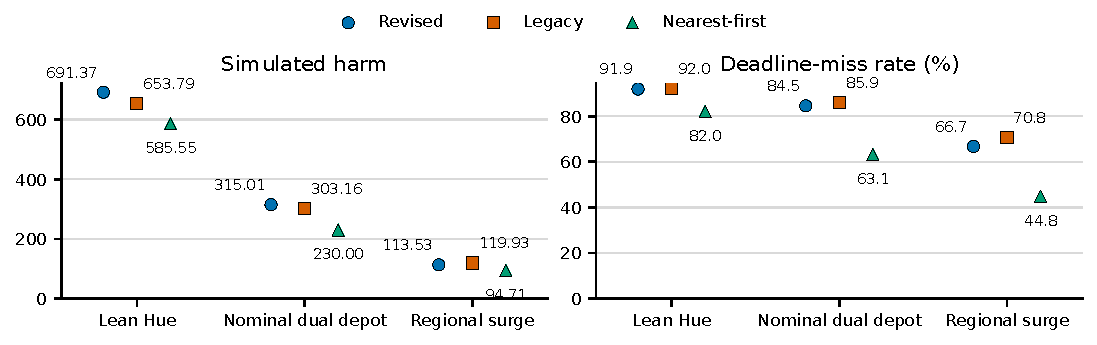
\includegraphics[width=\textwidth]{../paper/figures/rq3_dispatch_conditions.pdf}
\caption{Trung bình mô tả theo điều kiện nguồn lực trên phân hoạch Product}
\label{fig:rq3-conditions-report}
\end{figure}
\SourceNote{\RepoPath{paper/figures/rq3_dispatch_conditions.pdf}; mỗi điểm tổng hợp 40 seed trong một điều kiện. Phân tích chính dùng trung bình điều kiện trong seed và 40 cặp.}

Gần nhất trước có harm và trễ hạn trung bình thấp hơn trong mọi điều kiện được thử. Một diễn giải có thể là score theo nhu cầu chưa biểu diễn đủ chi phí đi lại và ràng buộc lịch; đây là giả thuyết giải thích, chưa được cô lập bằng thực nghiệm cơ chế. Kết quả không xác lập gần nhất trước là chính sách thực địa tối ưu.

\subsection{Luồng hệ thống và mạng yếu}
Lịch sử E2E ghi nhận chọn chế độ đúng khi dùng network throttling: mạng không giới hạn có ảnh gốc khoảng 53,6 KB, 300 kbit/s có ảnh nén khoảng 42,4 KB, 20 kbit/s chỉ gửi thông tin. Mất mạng/có mạng lại và báo cáo thiếu GPS cũng được kiểm tra ở luồng web. Các số kích thước này thuộc ảnh/kịch bản test cụ thể, không phải mức giảm trung bình trên một quần thể ảnh.

Script proxy mạng yếu hiện có ba hồ sơ 50/400/5.000 kbit/s với RTT 600/200/50 ms, cùng timeout metadata 30 giây và upload 60 giây. Repo không có bộ kết quả độ trễ tương ứng trong thư mục results để đưa vào bảng. Vì vậy, báo cáo có thể mô tả thiết kế phép đo và hành vi chức năng, nhưng chưa kết luận hệ thống rút ngắn thời gian phản ứng trong mạng di động thực.

\subsection{Bàn luận xuyên các tầng}
Các kết quả cho thấy cần đánh giá riêng ba dạng chất lượng: đúng biểu diễn tại thiết bị, đúng liên kết sự kiện và phù hợp quyết định điều phối. FP32 có parity tốt giữa runtime nhưng vẫn nhầm lớp; score có invariance exact nhưng alignment yếu; Product có chặn cạnh nhưng nhạy multiplicity. Không có một chỉ số đơn lẻ thay thế được các tầng còn lại.

Mức hoàn thành phần mềm tạo một nền tảng thử nghiệm có thể trình diễn và kiểm tra hợp đồng. Phần nghiên cứu thuật toán cung cấp các giới hạn toán học và kết quả âm có ích cho cải tiến. Khả năng ứng dụng được phát biểu ở mức nguyên mẫu hỗ trợ quyết định; hiệu quả cứu hộ ngoài thực tế còn cần dữ liệu độc lập, chuyên gia và thử nghiệm thiết bị/hạ tầng.
